% Homework 4.tex 

\documentclass{article}
\usepackage{graphicx} % for figures
\usepackage{float}
\usepackage[export]{adjustbox}
\begin{document}

\title{Homework Work 4 - Physics 240}
\author{Tin Tran}

\maketitle

\section{Introduction}

This is an excerise to calculate and plot the trajectory of a baseball using both the numerical and anaytical approach. The goal is to plot $y(x)$ versus time for the baseball.


\begin{figure}[H]
\centering{
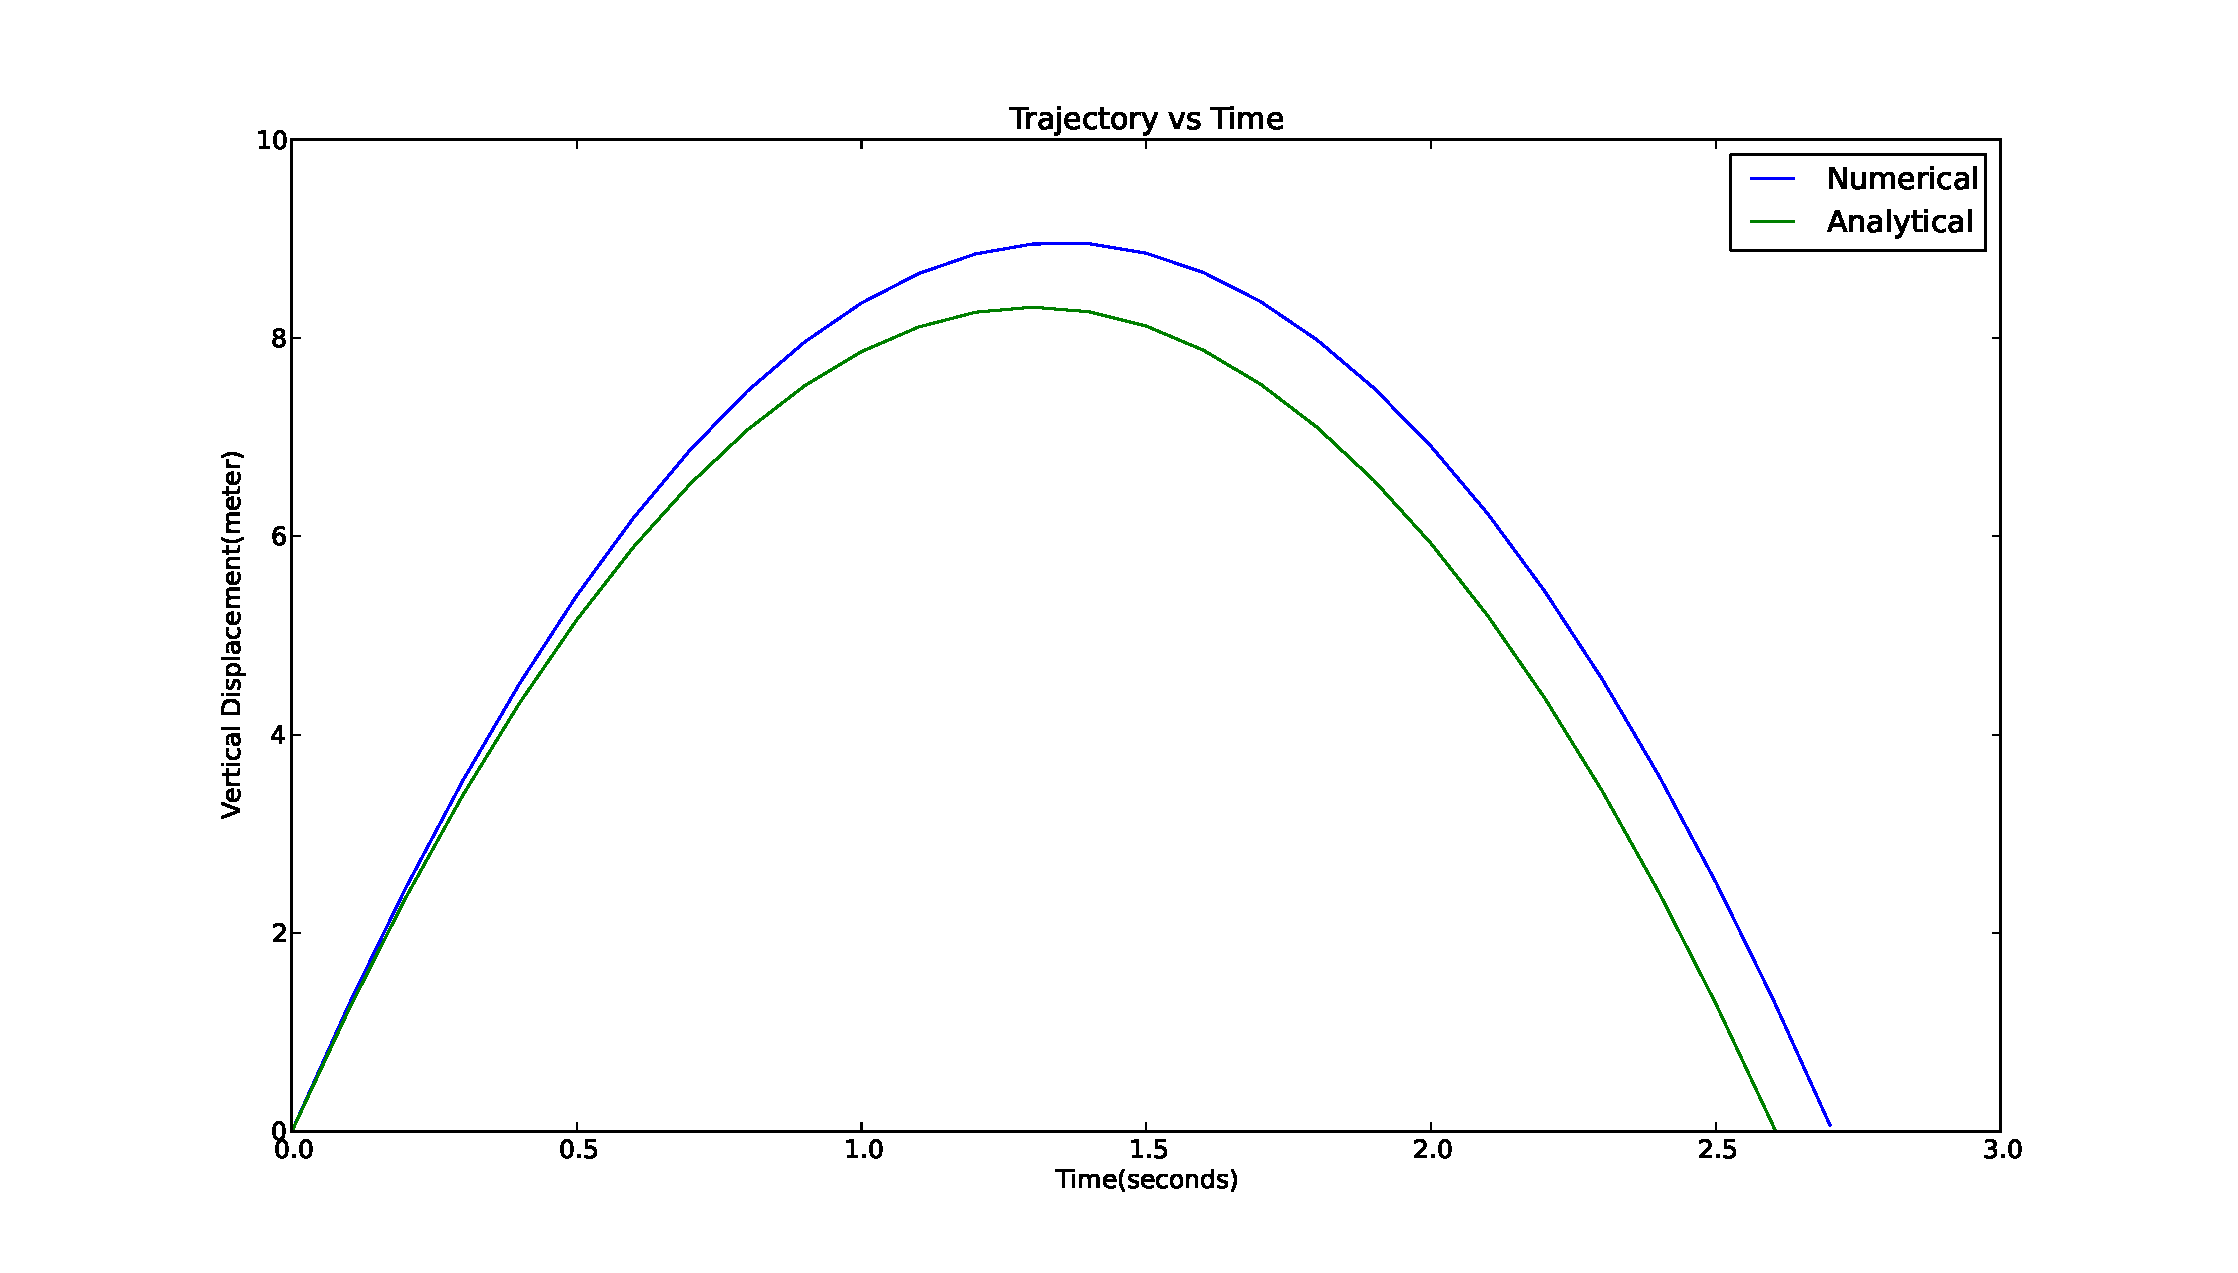
\includegraphics[max size={\textwidth}{\textheight}]{hw4.eps}
\caption{Numerical and Analytical solutions without air resistance}
}
\end{figure}
In figure(1) above, $v_0$ = 15 m/s, $\theta_0 = 45^0$, and $\Delta$t = 0.1 sec. This is without air resistance, the results of the range and flight time is showned below:  \\
Numerical range is:  22.0635\\
Numerical Flight time is:  2.8\\
Analytical range is:  22.0635\\
Analytical Flight time is:  2.8\\

I could not do the error analysis for the range and flight time because there is no difference for range is both values, so instead, I did the error analysis for the maximum hight instead. And the absoulte error for the maximum height of both solutions is 0.6393 $m$. Changing the value of $\Delta$t from 0.1 to 0.02 decrease this error to 0.12 $m$ or about 10 $cm$, which is what we want, and produces this plot below.
** Updated: There's something in my code, althouth the first plot shows the difference in the range, the values don't say so, and I still don't know why. I'm still keeping the $\Delta$t value.

\begin{figure}[H]
\centering{
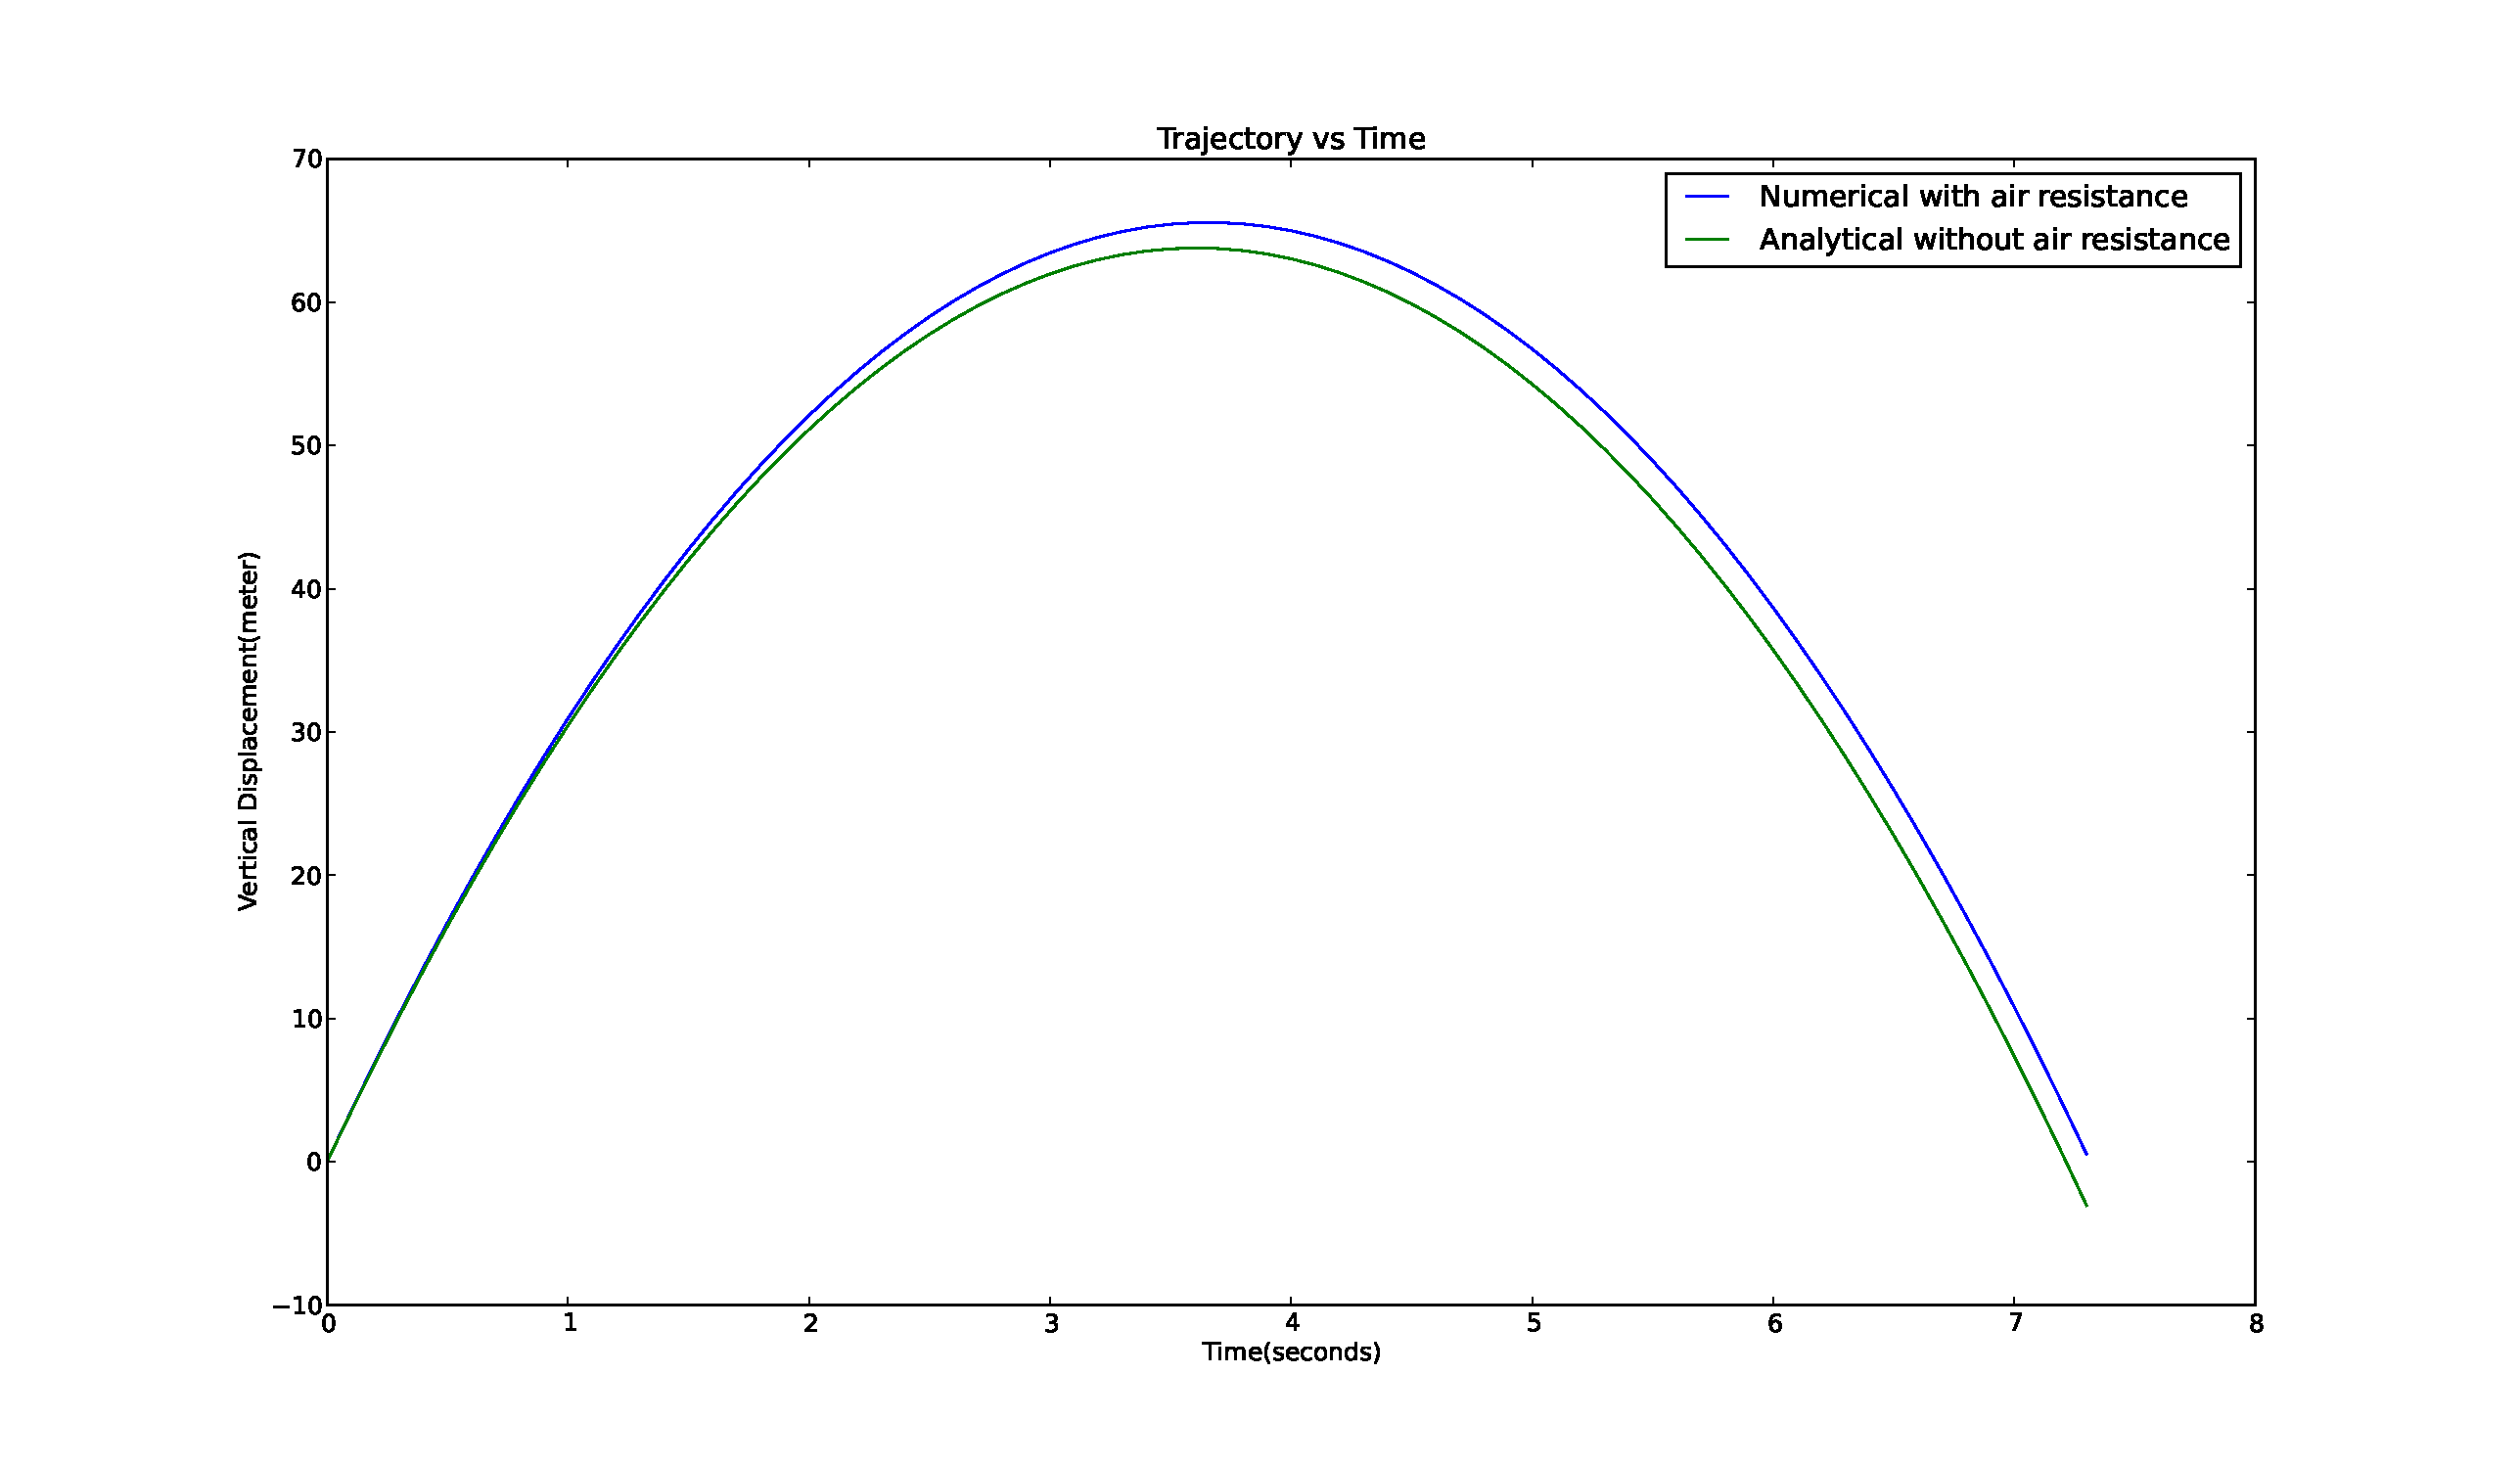
\includegraphics[max size={\textwidth}{\textheight}]{hw4er.eps}
\caption{Numerical and Analytical solutions without air resistance $\Delta$t = 0.02}
}
\end{figure}

\section{With Air resistance}
Using the new $\Delta$t value above, I now apply the air resistance into the equation, with $v_0$ = 50 $m/s$, drag coefficent $C_d$ = 0.35, air density = 1.2 $kg/m^3$, the cross-section area = 0.004 $m^2$, and the mass of the ball is 0.15 $kg$. The equation for air resistance is: \\
\indent \indent \indent $\vec{F}_a = \frac{-1}{2}C_d$$\rho A |\vec{v}|\vec{v}$\\
applying this air resistance factor into the equation, the results are shown in figure(3) below:
\begin{figure}[H]
\centering{
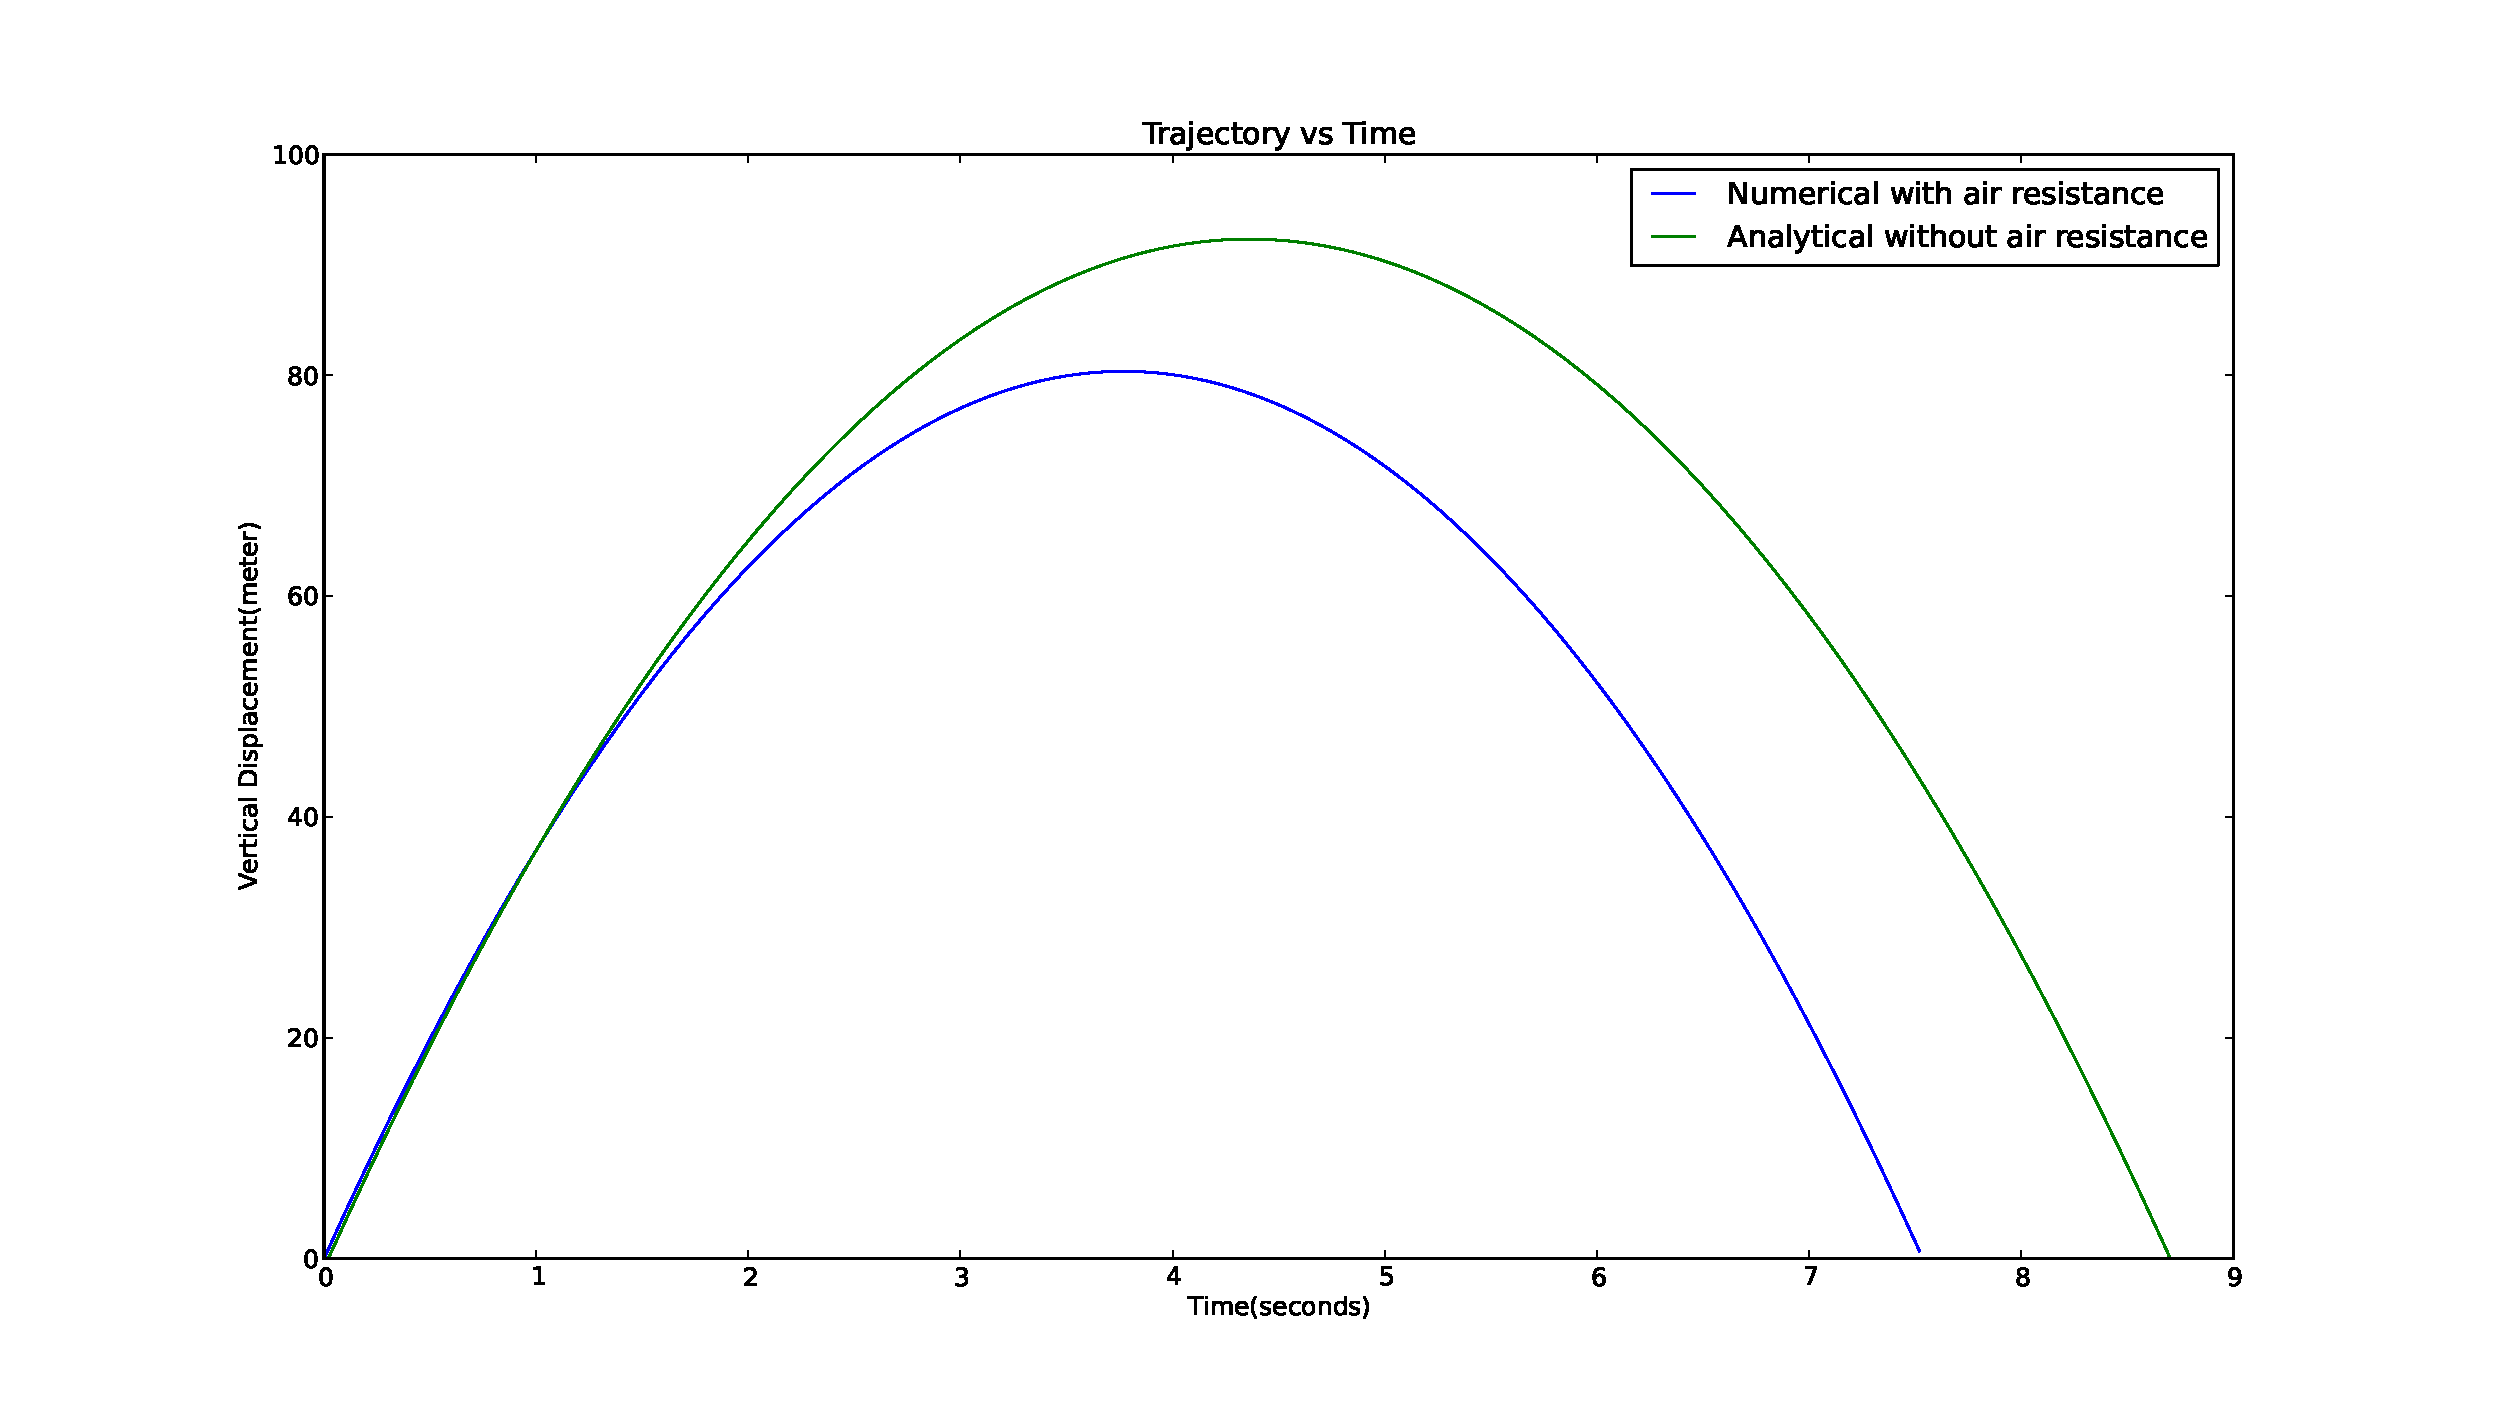
\includegraphics[max size={\textwidth}{\textheight}]{hw4s.eps}
\caption{Approximation using the new identity for $e^x$}
}
\end{figure}
And the results for the range and flight time is:\\
Numerical range with air resistance is:  198.046 $m$\\
Numerical Flight time with air resistance is:  7.54 $s$\\
Analytical range is:  229.040 $m$\\
Analytical Flight time is:  8.72 $s$\\

\end{document}